\documentclass[12pt]{article}
\usepackage{polski}
\usepackage[cp1250]{inputenc} % kodowanie polskich znak�w
\usepackage[T1]{fontenc}


\usepackage{color}
\usepackage{tikz}
\usetikzlibrary{arrows,positioning,shapes,calc,matrix}
\usepackage{pgf}
%\usepackage{lscape} % \begin{landscape} \end{landscape}
%\usepackage{pstricks}
\usepackage{geometry}

\geometry{hscale={0,88}}
\geometry{vscale={0,88}}

\title{Aktywacja kaspaz}
\date{}
\begin{document}
\maketitle
\bigskip
Schemat przedstawiaj�cy aktywacj� kaskady kaspaz w szlakach apoptotycznych.


\vspace{2cm}
\begin{tikzpicture}[node distance=2cm, auto]
\tikzset{
    %czubek strza�ki
    >=latex',
    %styl NODa
    punkt/.style={
           rectangle, rounded corners=4mm,
           inner sep=5pt,
           very thick,draw=black!50,
           top color=white,bottom color=black!20,
           %fill=lightgray!20,
           text width=6.5em,
           minimum height=2em,
           text centered}
}
%\draw[help lines,lightgray] grid (25,15);
%\Pola
\draw node[minimum height=10cm, rounded corners=6mm, minimum width=4cm, fill=red!20] (pole1) {};
\draw node[right=1cm of pole1, rounded corners=6mm, minimum height=10cm,minimum width=4cm,fill=blue!20] (pole2){};
\draw node[minimum height=10cm, right=1cm of pole2, rounded corners=6mm, minimum width=4.5cm, fill=red!50] (pole3) {};

%NODy
\node(kas8)  [punkt]                   {Kaspaza-8};
\node(sygnal)[left=2cm of kas8]        {\textbf{\textsc{{\Large Sygna�}}}};
\node(kas10) [punkt,below=3cm of kas8] {Kaspaza-10};
\node(kas9)  [punkt,above=3cm of kas8] {Kaspaza-9};

\node[punkt,right=2cm of kas9] (kas3) {Kaspaza-3};
\node[punkt,below=3cm of kas3] (kas6) {Kaspaza-6};
\node[punkt,below=3cm of kas6] (kas7) {Kaspaza-7};
\node[punkt,right=2cm of kas6] (rock) {Rock};
\node[right=1.7cm of kas7, text centered] (degradacja) {\textbf{\textsc{{\Large Degradacja}}}};

%Fazy
\node[below=1.5cm of kas10] (faza1) {\textbf{\textsc{{\LARGE Faza 1}}}};
\node[below=1.5cm of kas7] (faza2) {\textbf{\textsc{{\LARGE Faza 2}}}};
\node[right=2.6cm of faza2] (faza3) {\textbf{\textsc{{{\LARGE Faza 3}}}}};


%Strza�ki
\draw[->,very thick,shorten >=4pt, shorten <=4pt,dashed] (sygnal) -- (kas8);
\draw[->,very thick,shorten >=4pt, shorten <=4pt,dashed] (sygnal) -- (kas9.west);
\draw[->,very thick,shorten >=4pt, shorten <=4pt,dashed] (sygnal) -- (kas10.west);
\draw[->,very thick,shorten >=4pt, shorten <=4pt,] (kas8) -- (kas10);
\draw[->,very thick,shorten >=4pt, shorten <=4pt,] (kas8) -- (kas9);
\draw[->,very thick,shorten >=4pt, shorten <=4pt,] (kas8) -- (kas3.west);
\draw[->,very thick,shorten >=4pt, shorten <=4pt,] (kas8) -- (kas7.west);
\draw[->,very thick,shorten >=4pt, shorten <=4pt,dashed] (kas9) -- (kas7);
\draw[->,very thick,shorten >=4pt, shorten <=4pt,] (kas9) -- (kas3);
\draw[->,very thick,shorten >=4pt, shorten <=4pt,] (kas10) -- (kas3);
\draw[->,very thick,shorten >=4pt, shorten <=4pt,] (kas10) -- (kas7);
\draw[<->,very thick,shorten >=4pt, shorten <=4pt,] (kas7) -- (kas6);
\draw[<->,very thick,shorten >=4pt, shorten <=4pt,] (kas6) -- (kas3);
\draw[->,very thick,shorten >=4pt, shorten <=4pt,dashed] (kas6) -- (rock);
\draw[->,very thick,shorten >=4pt, shorten <=4pt,dashed] (kas7) -- (rock.west);
\draw[->,very thick,shorten >=4pt, shorten <=4pt,dashed] (kas3) -- (rock.west);
\draw[->,very thick,shorten >=4pt, shorten <=4pt,dashed] (kas3) -- (rock.west);
\draw[->,very thick,shorten >=4pt, shorten <=4pt,dashed] (rock) -- (degradacja);
\end{tikzpicture}

\newpage
\begin{center}
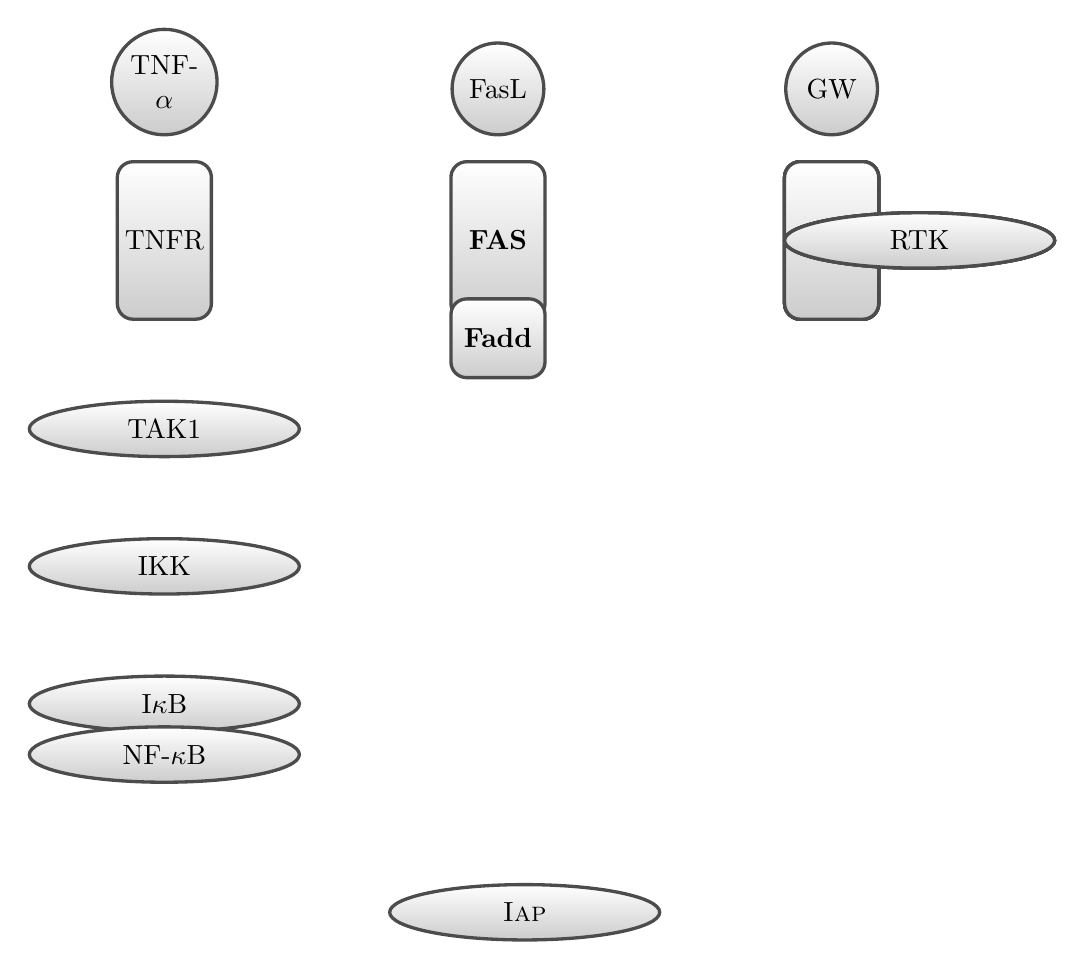
\begin{tikzpicture}[node distance=2cm, auto]
\tikzset{
    %czubek strza�ki
    >=latex',
    %styl NODa
    punkt/.style={
           rectangle, rounded corners=2mm,
           inner sep=2pt,
           very thick,draw=black!70,
           top color=white,bottom color=black!20,
           %fill=lightgray!20,
           text width=3em,
           minimum height=2cm,
           text centered},
    punktg/.style={
           ellipse, rounded corners=4mm,
           inner sep=2pt,
           very thick,draw=black!70,
           top color=white,bottom color=black!20,
           %fill=lightgray!20,
           text width=6.5em,
           minimum height=2em,
           text centered},
    diament/.style={
           diamond, rounded corners=.4mm,
           inner sep=2pt,
           very thick,draw=black!70,
           top color=white,bottom color=black!20,
           %fill=lightgray!20,
           text width=2.5em,
           minimum height=2em,
           text centered},
    kolo/.style={
           circle, rounded corners=4mm,
           inner sep=1pt,
           very thick,draw=black!70,
           top color=white,bottom color=black!20,
           %fill=lightgray!20,
           text width=3em,
           minimum height=2em,
           text centered}
}
%NODy


\node(fas)       [punkt]                     {\textbf{FAS}};
\node(tnfr)      [punkt,left=3cm of fas]     {TNFR};
\node(rtk)       [punkt,right=3cm of fas,minimum height=2cm]    {RTK};
\node(tnf)       [kolo,above=.3cm of tnfr]   {TNF-$\alpha$};
\node(fasl)      [kolo,above=.3cm of fas]    {FasL};
\node(gw)        [kolo,above=.3cm of rtk]    {GW};

%Sciezka TNFR
\node(fadd)      [punkt,below=-.3cm of fas,minimum height=1cm,minimum width=.7cm]    {\textsc{\textbf{Fadd}}};
\node(tak1)      [punktg,below=1cm of tnfr]    {TAK1};
\node(ikk)       [punktg,below=1cm of tak1]    {IKK};
\node(ikb)       [punktg,below=1cm of ikk]    {I$\kappa$B};
\node(nfkb)      [punktg,below=-.1cm of ikb]    {NF-$\kappa$B};
\node(iap)       [punktg,below right=3cm of ikb]    {\textsc{Iap}};


%Sciezka FAS

\node(pi3k)      [punkt,right=3cm of fas]    {RTK};
\node(akt)       [punkt,right=3cm of fas]    {RTK};
\node(bad)       [punkt,right=3cm of fas]    {RTK};
\node(gsk)       [punkt,right=3cm of fas]    {};
\node(akt)       [punkt,right=3cm of fas]    {RTK};
\node(bad)       [punkt,right=3cm of fas]    {RTK};

\node(kaz367)    [punktg,right=3cm of fas]    {RTK};
\node(kaz810)    [punktg,right=3cm of fas]    {RTK};
\node(ikb)       [punktg,right=3cm of fas]    {RTK};
\node(nfkb)      [punktg,right=3cm of fas]    {RTK};

%
%\node(bcl2)      [diament,left=1cm of bad]                 {Bcl-XL};
%\node(bclxl)     [diament,left=.1cm of bcl2]         {Bcl-2};
%\node(puma)     [diament,left=.1cm of bclxl]         {Puma};
%\node(noxa)     [diament,left=.1cm of bax]         {Noxa};

%\node(akt)     [kolo,right=.1cm of bax]         {Akt};
%\node(cath)    [punkt]                                    {Cathepsin};
%
%\node(bh3)     [punkt,above=2cm of cath]                  {BH-3 only};
%\node(bcl2)    [punkt,right=1cm of cath]                  {Bcl-2};

%\node(ptp)     [draw,very thick,right=1.8cm of bcl2,ellipse,dashed]  {\textbf{{\Large PTP}}};
%\node(cytc)    [below=3cm of bcl2]                        {\textbf{{\LARGE Cyt C}}};
%\node(apaf1)   [punkt,left=1cm of cytc]                   {Apaf-1};
%\node(+)       [left=0.1 of cytc]                       {\textbf{{\LARGE +}}};
%\node(cas9)    [punkt,below=1cm of cytc]                  {Caspase-9};
%\node(cas37)    [punkt,below=1cm of cas9]                  {Caspase-3/7};
%\node(degr)    [below=1cm of cas37]                        {\textbf{\textsc{Degradation}}};
%
%%Strza�ki
%\draw[-|,very thick,shorten >=4pt, shorten <=4pt] (cath) -- (bcl2);
%\draw[-|,very thick,shorten >=4pt, shorten <=4pt] (bcl2) -- (bax.west);
%\draw[-|,very thick,shorten >=4pt, shorten <=4pt] (bcl2) -- (bak.west);
%\draw[->,very thick,shorten >=4pt, shorten <=4pt] (bak) -- (ptp);
%\draw[->,very thick,shorten >=4pt, shorten <=4pt] (bax) -- (ptp);
%\draw[-|,very thick,shorten >=4pt, shorten <=4pt] (bh3) -- (bcl2.north west);
%\draw[->,very thick,shorten >=4pt, shorten <=4pt,dashed] (ptp) .. controls +(right:6cm) and +(right:2cm) .. (cytc);
%\draw[->,very thick,shorten >=4pt, shorten <=4pt] (cytc) -- (cas9);
%\draw[->,very thick,shorten >=4pt, shorten <=4pt] (cas9) -- (cas37);
%\draw[->,very thick,shorten >=4pt, shorten <=4pt] (cas37) -- (degr);
\end{tikzpicture}
\end{center}
\end{document}
